%************************************************
\chapter{Development}
\label{ch:Development}
%************************************************

\section{Introduction}
\label{sec:dev_introduction}

This chThe implementation follows the general TimesNet framework with battery-specific improvements:

\begin{itemize}
    \item \textbf{Sequence length}: Fixed-length sequences of 100 time steps were used to capture enough time context while keeping computation efficient.
    \item \textbf{Period discovery}: The FFT-based period detection was applied to identify natural cycles in battery operation, such as charge-discharge patterns and longer-term capacity fade cycles.
    \item \textbf{2D data processing}: The inception blocks were set up with appropriate filter sizes to capture multi-scale time changes relevant to battery degradation processes.
    \item \textbf{Combination weights}: The amplitude-based combination mechanism was used to automatically weight different periodic components based on their importance in the frequency analysis.
\end{itemize}tails the development phases of the battery health prediction system, covering the complete progress from initial MATLAB modeling to advanced deep learning implementation. The project evolved through distinct phases: (1) MATLAB-based modeling and simulation using traditional methods, (2) exploration of hybrid neural network approaches, (3) transition to pure data-driven models, and (4) implementation of state-of-the-art deep learning architectures for time series forecasting.

The development process was guided by the need to create accurate, strong, and scalable battery health prediction models capable of handling real-world applications. Each phase built upon lessons learned from previous approaches, ultimately leading to the implementation of TimesNet, a cutting-edge time series analysis architecture that demonstrates superior performance in battery degradation prediction tasks.

\section{MATLAB Modeling and Simulation}
\label{sec:matlab_modeling}

The initial development phase focused on implementing traditional battery modeling approaches in MATLAB to establish baseline performance and understand the basic characteristics of battery degradation patterns.

\textbf{Kalman Filter Implementation}
\label{subsec:kalman_filter}

The Extended Kalman Filter (EFK) was implemented as the primary estimation algorithm for SOC and SOH prediction. The EFK approach was chosen for its proven effectiveness in handling the nonlinear behavior of battery systems and its ability to provide uncertainty measurement.

\textbf{Coulomb Counting Integration}
\label{subsec:coulomb_counting}

Coulomb counting was integrated as a supporting method for SOC estimation, providing a reference baseline for comparison with the Kalman filter results. The implementation addressed several critical considerations to ensure accuracy and reliability. \textbf{Current integration accuracy and drift compensation} were prioritized to minimize cumulative errors that could significantly impact SOC estimates over extended periods. \textbf{Temperature effects on coulombic efficiency} were carefully analyzed, as thermal variations can substantially alter the charge-discharge efficiency and affect the accuracy of capacity calculations. \textbf{Aging effects on capacity estimation} were incorporated to account for the gradual degradation of battery capacity over operational lifetime, ensuring that SOC estimates remain accurate as the battery ages. Finally, \textbf{calibration procedures for initial SOC determination} were established to provide accurate baseline measurements, which are crucial for the cumulative nature of coulomb counting methods.

\textbf{Batemo Model Integration}
\label{subsec:batemo_model}

The Batemo battery model was incorporated to provide physics-based battery behavior simulation. This integration offered complete capabilities for model development and validation. \textbf{Validation of estimation algorithms under controlled conditions} was enabled through the model's ability to simulate precise battery behaviors, allowing for systematic testing of algorithm performance across various operational scenarios. \textbf{Generation of synthetic data for algorithm testing} provided a valuable resource for training and evaluating neural networks when real-world data was limited or when specific degradation patterns needed to be studied. \textbf{Analysis of model sensitivity to various degradation mechanisms} was made possible by the physics-based nature of the Batemo model, enabling detailed investigation of how different aging phenomena affect battery performance predictions. Additionally, \textbf{comparison between model-based and data-driven approaches} was made possible, allowing for complete evaluation of different estimation methodologies and their respective strengths and limitations.

The MATLAB implementation served as a foundation for understanding battery dynamics and provided insights that informed subsequent neural network development phases.

\section{Neural Network Development Evolution}
\label{sec:neural_network_evolution}

The neural network development process evolved through multiple iterations, each addressing specific limitations identified in previous approaches and incorporating lessons learned from the MATLAB modeling phase.

\textbf{Initial CNN+LSTM Architecture}
\label{subsec:cnn_lstm_architecture}

The first neural network implementation combined CNN with LSTM networks to leverage both spatial feature extraction and temporal sequence modeling capabilities.

\textbf{Architecture Design}

The CNN+LSTM architecture was structured to use the supporting strengths of both convolutional and recurrent neural networks. The design incorporated multiple specialized layers, each serving a distinct purpose in the feature extraction and temporal modeling pipeline. \textbf{CNN layers} were responsible for extracting local patterns and features from battery measurement sequences, identifying spatial relationships and important signal characteristics within the input data. \textbf{LSTM layers} focused on modeling long-term dependencies and temporal relationships, capturing the sequential nature of battery degradation and state evolution over time. Finally, \textbf{Dense layers} provided the final prediction mapping with appropriate activation functions, transforming the processed features into accurate SOC and SOH estimates.

\textbf{Training Challenges and Limitations}

Several significant challenges were encountered during the CNN+LSTM implementation that highlighted the complexity of applying deep learning to battery health monitoring. These obstacles required careful analysis and ultimately influenced the decision to pursue alternative approaches. \textbf{Gradient vanishing} emerged as a critical issue where long sequences caused training instability, preventing the network from effectively learning long-term dependencies essential for accurate battery state prediction. \textbf{Overfitting} presented another major concern, as the high model complexity led to poor generalization, with the network memorizing training patterns rather than learning transferable features applicable to new battery data. \textbf{Computational efficiency} posed practical limitations, with training time becoming too long for large datasets, making the approach unsuitable for real-world applications requiring timely model updates. Additionally, \textbf{Feature engineering} proved challenging, as manual feature selection proved suboptimal, requiring extensive domain expertise and iterative refinement that limited the model's adaptability to different battery types and operating conditions.

\textbf{Hybrid vs. Data-Driven Approach Evaluation}
\label{subsec:hybrid_vs_datadriven}

A systematic comparison was conducted between hybrid approaches (combining physics-based models with neural networks) and pure data-driven methods.

\textbf{Hybrid Approach Implementation}

The hybrid approach integrated multiple supporting techniques to use both physics-based understanding and data-driven learning capabilities. This complete strategy incorporated several key components designed to enhance prediction accuracy and reliability. \textbf{Physics-based model outputs as additional input features} provided domain-specific insights that enriched the neural network's understanding of battery behavior, incorporating basic electrochemical principles into the learning process. \textbf{Kalman filter estimates as regularization terms} helped constrain the neural network training by incorporating well-established state estimation techniques, reducing the likelihood of unrealistic predictions and improving model stability. Furthermore, \textbf{domain knowledge constraints in loss function design} ensured that the learned models respected known physical limitations and relationships, preventing the network from learning patterns that violated basic battery physics principles.

\textbf{Data-Driven Approach Focus}

The pure data-driven approach emphasized maximum use of machine learning capabilities while minimizing reliance on explicit domain knowledge. This methodology focused on allowing the neural network to discover patterns and relationships directly from the data. \textbf{End-to-end learning from raw sensor data} enabled the model to process unfiltered battery measurements, potentially capturing subtle patterns that might be lost during manual preprocessing or feature engineering steps. \textbf{Automatic feature extraction and representation learning} allowed the network to identify the most relevant characteristics for battery health prediction without requiring extensive domain expertise or manual feature design. Additionally, \textbf{minimal domain-specific preprocessing requirements} reduced implementation complexity and improved the method's adaptability to different battery types and measurement configurations, making it more suitable for diverse real-world applications.

\textbf{Comparative Analysis Results}

The evaluation revealed that data-driven approaches demonstrated \textbf{better generalization} across different battery chemistries, \textbf{reduced dependency} on accurate physics model parameters, \textbf{better scalability} to large datasets, and \textbf{more strong performance} under varying operating conditions.

This analysis motivated the transition to advanced pure data-driven architectures.

\section{Dataset Collection and Preprocessing}
\label{sec:dataset_preprocessing}

The dataset development process was crucial for training strong and generalizable models, requiring careful consideration of data quality, diversity, and preprocessing strategies.

\textbf{Primary Dataset Selection}
\label{subsec:primary_dataset}

The primary dataset used in this work is the CALCE (Center for Advanced Life Cycle Engineering) battery dataset, obtained from the University of Maryland's public repository. This dataset was selected for its:

\begin{itemize}
    \item Complete cycle life data spanning multiple battery chemistries
    \item High-quality measurements with consistent sampling rates
    \item Well-documented experimental conditions and procedures
    \item Established use in battery research community for benchmarking
\end{itemize}

\textbf{Data Cleaning and Preprocessing}

Several preprocessing steps were implemented to ensure data quality and model training stability:

\textbf{Cycle Removal and Filtering}

\begin{itemize}
    \item \textbf{Initial cycle removal}: The first charge-discharge cycle was removed from each battery file to avoid initialization artifacts and inconsistent starting conditions
    \item \textbf{Incomplete cycle filtering}: Cycles with insufficient data points or incomplete charge/discharge sequences were excluded from the training set
    \item \textbf{Outlier detection}: Statistical methods were applied to identify and remove measurement outliers that could negatively impact model training
\end{itemize}
Battery-level partitioning was employed to prevent data leakage, ensuring that cycles from the same battery appeared in only one partition.

\textbf{Input Data Formatting}

The input data structure was designed to optimize model performance:

\begin{itemize}
    \item \textbf{Sequence length}: Fixed-length sequences of 100 time steps were extracted from continuous battery operation data
    \item \textbf{Feature vector}: Each time step included voltage, current, temperature, and derived features such as power and energy
    \item \textbf{Target variables}: State of Health (SOH) values were calculated based on capacity fade measurements
    \item \textbf{Sliding window}: Overlapping sequences were generated to maximize training data utilization
\end{itemize}

\textbf{Limitations of Previous Approaches}

The evaluation of CNN+LSTM and hybrid approaches revealed several critical limitations:

\begin{itemize}
    \item \textbf{Temporal modeling constraints}: Traditional LSTM architectures struggled with very long sequences typical in battery degradation analysis
    \item \textbf{Multi-scale pattern recognition}: Difficulty in capturing both short-term fluctuations and long-term degradation trends simultaneously
    \item \textbf{Computer efficiency}: High computer requirements limited the scalability to large datasets
    \item \textbf{Generalization issues}: Poor performance when applied to battery chemistries or operating conditions not seen during training
\end{itemize}

\textbf{Requirements for Advanced Architecture}

The identified requirements for an improved architecture included:

\begin{itemize}
    \item \textbf{Multi-periodicity detection}: Ability to automatically identify and exploit multiple periodic patterns in battery data
    \item \textbf{Long-range dependency modeling}: Effective capture of dependencies across extended time horizons
    \item \textbf{Parameter efficiency}: Reduced model complexity while maintaining or improving performance
    \item \textbf{Versatility}: Capability to handle various time series analysis tasks beyond just forecasting
\end{itemize}

These requirements led to the selection and implementation of TimesNet, a cutting-edge architecture specifically designed for general time series analysis.

\section{Utilized Model (TimesNet)}
\label{sec:timesnet_model}

TimesNet is a modern neural network designed specifically for analyzing time series data~\cite{wu_timesnet_2023}. This model tackles the basic challenge of understanding how data changes over time by converting the complex problem from analyzing 1D time series into analyzing 2D patterns. The key innovation of TimesNet is its ability to discover repeating patterns (periodicity) in time series data and break down complex time changes into smaller, more manageable pieces.

\textbf{Multi-Periodicity Analysis}

TimesNet starts by analyzing the time series in the frequency domain using Fast Fourier Transform (FFT) to discover multiple periods. Real-world time series usually present multi-periodicity, such as daily and yearly variations for weather observations, or weekly and quarterly variations for electricity consumption. 

The period discovery process works by analyzing the frequency spectrum of the input data. The algorithm calculates the amplitude of different frequencies and identifies the strongest periodic patterns by selecting the top-k frequencies with the highest amplitudes. These dominant frequencies correspond to the most important periodic behaviors in the data, such as charge-discharge cycles in battery operations or longer-term capacity fade patterns.

\textbf{2D Transformation Process}

The architecture works by converting 1D time series into a set of 2D grids based on multiple identified periods. This transformation organizes patterns within each period into columns and patterns across different periods into rows of the 2D grids, making time patterns easier to analyze using 2D image processing techniques. 

Based on the selected frequencies and corresponding period lengths, the 1D time series is reshaped into multiple 2D tensors. This process takes the original time series data and reorganizes it into a grid-like format where each period becomes a row and the progression through different periods becomes columns.

The reshaping process essentially converts temporal patterns into spatial patterns that can be analyzed using 2D image processing techniques. Each identified period creates a separate 2D representation of the data, allowing the model to examine patterns at different time scales simultaneously.

Figure~\ref{fig:timesnet_2d_transformation} illustrates this transformation process, showing how discovering periodicity enables the conversion of original 1D time series into structured 2D tensors that can be processed by 2D kernels conveniently. 

\textbf{TimesBlock Architecture}

The core component, TimesBlock, can automatically discover multiple periods and extract complex time patterns using efficient inception blocks. Each TimesBlock works in a way that preserves the original signal while adding new information, and consists of two main parts:

\begin{enumerate}
\item \textbf{Capturing time patterns in 2D}: After converting the 1D time series into multiple 2D grids, each grid is processed by an efficient inception block that uses different sized filters. This design allows the model to examine patterns at multiple scales - both within individual periods (columns) and across different periods (rows) at the same time.

\item \textbf{Adaptive aggregation}: The k different processed features are combined based on their corresponding amplitudes of the estimated periods. The model uses a weighted combination where stronger periodic patterns (higher amplitudes) have more influence on the final result. This adaptive weighting ensures that the most important temporal patterns dominate the model's predictions.
\end{enumerate}

The shared inception block design makes the model size stay the same regardless of how many periods k are selected, improving efficiency.

\begin{figure}[htbp]
    \centering
    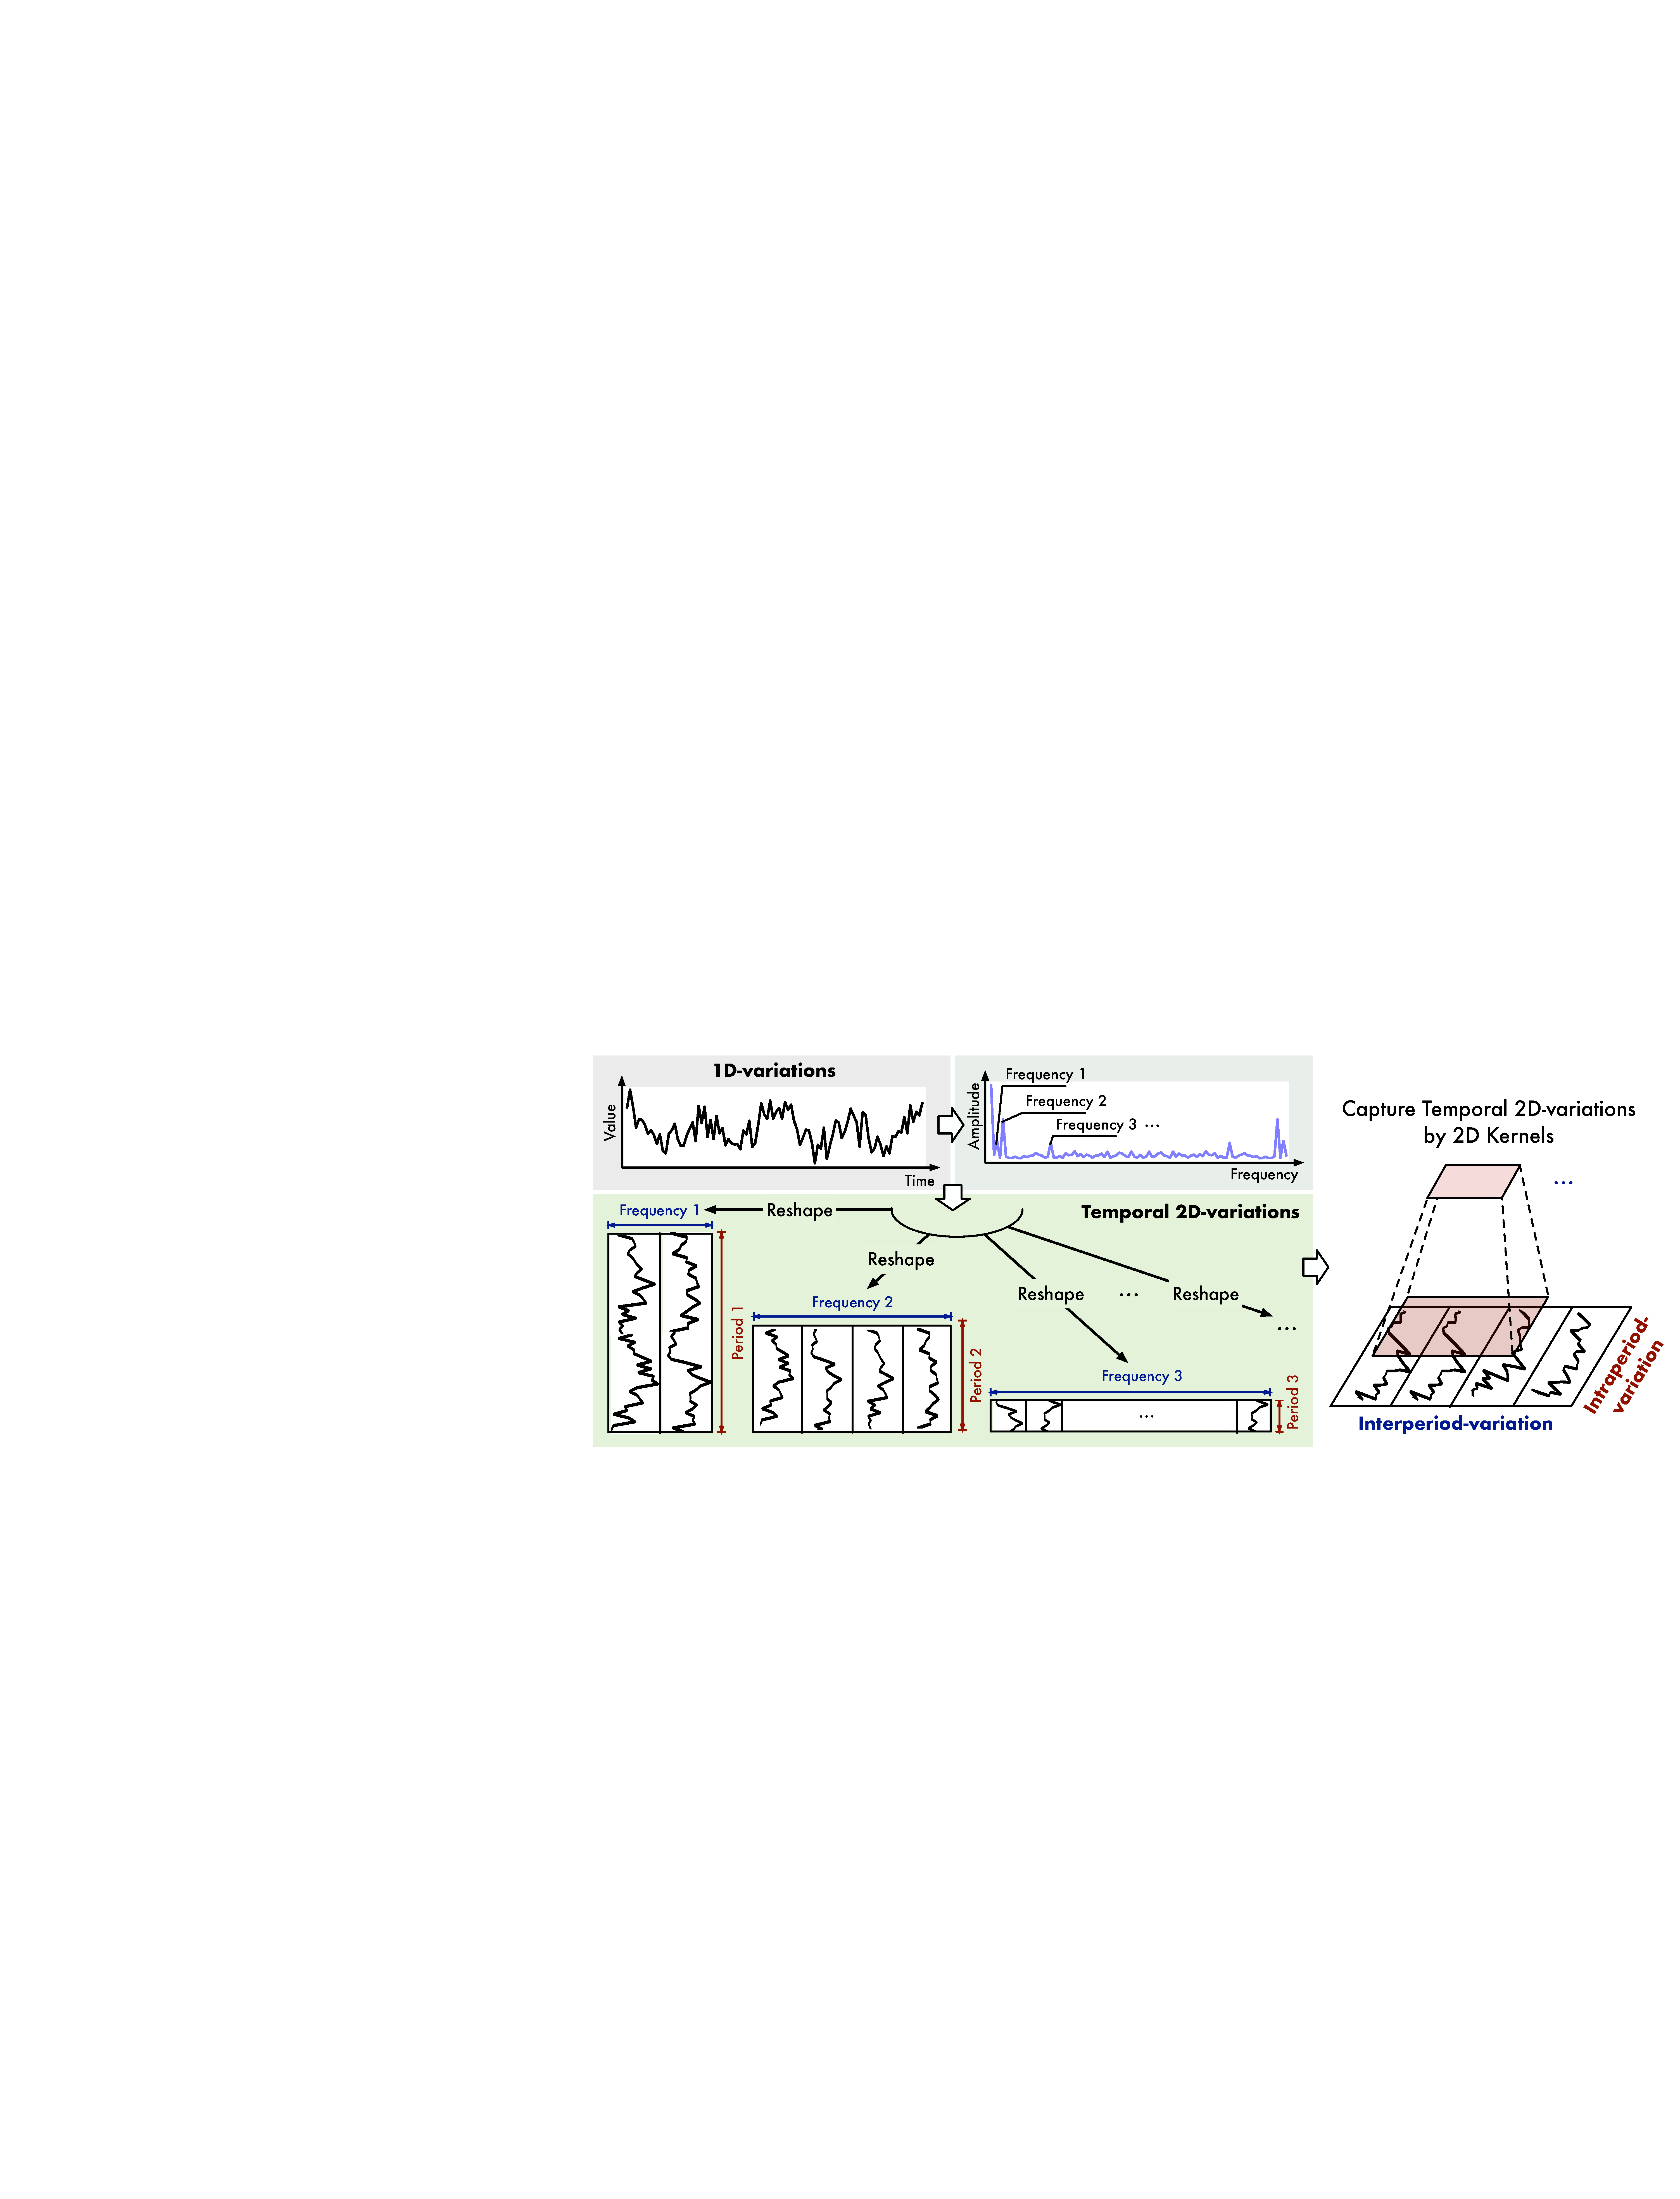
\includegraphics[width=0.8\textwidth]{imgs/timesnet_2d_structure.pdf}
    \caption{TimesNet 2D transformation: converting 1D time series into structured 2D tensors by discovering periodicity~\cite{wu_timesnet_2023}.}
    \label{fig:timesnet_2d_transformation}
\end{figure}

TimesNet shows better performance across five main time series analysis tasks: short-term and long-term forecasting, filling in missing data, classification, and anomaly detection. This flexibility makes it particularly suitable for battery health prediction tasks, where complex time dependencies and patterns at multiple scales are crucial for accurate state-of-health estimation. 

\textbf{Advantages for Battery Applications}

The model's ability to handle various sequence lengths and its strong design for capturing time dynamics work well with the requirements of battery degradation modeling, where both short-term changes and long-term trends must be considered at the same time. Key advantages include:

\begin{itemize}
\item \textbf{Multi-scale time modeling}: The 2D transformation allows capturing both short-term battery behavior (within periods) and long-term degradation trends (across periods) at the same time.
\item \textbf{Automatic period detection}: The FFT-based period discovery can identify natural cycles in battery operation without manual setup.
\item \textbf{Efficiency}: The shared inception block design keeps the model compact while handling multiple time scales.
\item \textbf{Flexibility}: The general-purpose nature allows adaptation to different battery types and operating conditions.
\end{itemize}

Unlike previous methods that struggle with the complex time patterns in battery data, TimesNet's 2D approach makes time changes easier to analyze. The transformation breaks the limitation of representation ability in the original 1D space, enabling more effective modeling of complex battery degradation patterns.

\textbf{Architecture Adaptation for Battery Health Prediction}
\label{subsec:timesnet_adaptation}

The TimesNet architecture was adapted for battery health prediction with several key modifications to optimize performance for this specific domain:

\begin{itemize}
    \item \textbf{Input preprocessing}: Battery measurement sequences (voltage, current, temperature) were formatted to exploit the multi-periodicity detection capabilities. The input sequences were structured to capture both charge-discharge cycles and longer-term aging patterns.
    \item \textbf{Output configuration}: Modified for regression tasks to predict continuous SOH values rather than classification outputs. The final layer was adapted to output single scalar values representing battery health percentages.
    \item \textbf{Loss function}: Used Mean Squared Error (MSE) with additional rules to prevent overfitting and ensure stable training.
    \item \textbf{Feature engineering}: Minimal manual feature creation to use the model's automatic pattern discovery abilities. This approach allows TimesNet to automatically identify relevant time patterns in battery data without requiring specialized feature design.
    \item \textbf{Period selection}: The top-k parameter was optimized specifically for battery data characteristics, allowing the model to focus on the most relevant repeating patterns in battery operation and degradation cycles.
\end{itemize}

\textbf{Technical Implementation Details}

The implementation follows the general TimesNet framework with battery-specific optimizations:

\begin{itemize}
    \item \textbf{Sequence length}: Fixed-length sequences of 100 time steps were used to capture sufficient temporal context while maintaining computational efficiency.
    \item \textbf{Period discovery}: The FFT-based period detection was applied to identify natural cycles in battery operation, such as charge-discharge patterns and longer-term capacity fade cycles.
    \item \textbf{2D tensor processing}: The inception blocks were configured with appropriate kernel sizes to capture multi-scale temporal variations relevant to battery degradation processes.
    \item \textbf{Aggregation weights}: The amplitude-based aggregation mechanism was used to automatically weight different periodic components based on their importance in the frequency domain.
\end{itemize}

\section{Model Optimization}
\label{sec:model_optimization}

For model optimization, the Optuna tool was utilized, which enables hyperparameter optimization for machine learning models, integrated with Weights \& Biases (WandB), which allows for result visualization and model comparison.

\textbf{Dataset Preparation for Optimization}

For this test, the dataset was reduced to only 1/10 of the data, equally distributed from the original dataset, with the objective of reducing the time required for finding the best hyperparameters, since this process took approximately one week even with this reduction.

\textbf{Optimization Process}
\label{subsec:optimization_process}

For the hyperparameter search, 50 trials were performed, with 50 epochs each, using an early stopping patience of 5 epochs to avoid overfitting and accelerate the optimization process.

\textbf{Optimized Parameters}

The parameters that were optimized through Optuna include:

\begin{itemize}
    \item \textbf{e\_layers}: Number of encoder layers (1--3) --- controls the depth of the encoder stack
    \item \textbf{d\_layers}: Number of decoder layers (1--3) --- controls the depth of the decoder stack  
    \item \textbf{factor}: Expansion factor for the FFN (1--5) --- controls the complexity of frequency components in TimesNet
    \item \textbf{freq}: Frequency for time features encoding (``s'', ``t'', ``h'') --- seconds, minutes, hours
    \item \textbf{d\_model}: Model dimension (fixed at 16)
    \item \textbf{top\_k}: Top-k dominant frequencies in TimesNet (1--5) --- controls how many frequency components to consider
\end{itemize}

\textbf{Parameter Importance Analysis}

Through this optimization, it was possible to detect the importance of the hyperparameters. The analysis showed that the importance factor of the \textbf{e\_layers} parameter (number of encoder layers) is the parameter that most influences the result when changed, demonstrating that the depth of the encoder architecture is critical for model performance.

\textbf{Best Trial Results}
\label{subsec:best_trial_results}

The most successful trial was trial 15, which presented the following results:

\begin{itemize}
    \item \textbf{MSE Value}: 0.0015545075293630362
    \item \textbf{Optimal Parameters}:
    \begin{itemize}
        \item e\_layers: 2
        \item factor: 4  
        \item d\_model: 16
        \item top\_k: 9
        \item n\_heads: 16
    \end{itemize}
    \item \textbf{Duration}: 7770232 ms (approximately 2 hours and 10 minutes)
\end{itemize}

The results show that using 2 encoder layers works better than deeper networks, likely avoiding overfitting on the battery dataset. The high expansion factor of 4 allows the model to capture more complex patterns, while setting top\_k to 9 means the model considers more frequency components than the default range, which helps capture the various periodic behaviors in battery degradation cycles.

\section{Experiments and Results}
\label{sec:experiments_results}

\lipsum[2-4]

\section{Conclusion and Future Work}
\label{sec:conclusion_future_work}
\lipsum[1]
\subsection{Conclusion}
\lipsum[5-6]
\subsection{Future Work}
\lipsum[7-8]


